\documentclass[amsmath,amssymb,aps,prd,10pt,twocolumn,showkeys]{revtex4}
\usepackage{graphicx}
\usepackage{mathtools}
\usepackage{verbatim}
\DeclareMathOperator\erfc{erfc}
\DeclareMathOperator\erf{erf}
\DeclareMathOperator{\sgn}{sgn}
\DeclareMathOperator{\snr}{SNR}
\begin{document}

\title{Complex Analysis of Askaryan Radiation: UHE-$\nu$ Identification and Reconstruction via the Hilbert Envelope of Observed Signals}

\author{Jordan C. Hanson}
\email{jhanson2@whittier.edu}
\affiliation{Department of Physics and Astronomy, Whittier College}
\author{Raymond Hartig}
\affiliation{Department of Physics and Astronomy, Whittier College}
\date{\today}

\begin{abstract}
The detection of ultra-high energy neutrinos (UHE-$\nu$), with enegies above 10 PeV, has been a long-time goal in astroparticle physics.  Autonomous, radio-frequency (RF) UHE-$\nu$ detetectors have been deployed in polar regions.  These detectors rely on the Askaryan effect in ice for the neutrino signal.  The Askaryan effect occurs when the excess negative charge within a high-energy cascade radiates in a dense medium.  UHE-$\nu$ can induce such cascades that radiate in the RF bandwidth above thermal backgrounds.  To identify UHE-$\nu$ signals in data from Askaryan-class detectors, analytic models of the Askaryan electromagnetic field have been created and matched to simulations and laboratory measurements.  These models have correctly described the Askaryan electromagnetic field, but leave the effects of attenuation from signal propagation through polar ice and RF channel response to simulation packages.  In this work, a fully analytic Askaryan model that accounts for these effects is presented.  First, formulas for the observed voltage trace and its Hilbert envelope are calculated.  Second, the analytic model is compared to UHE-$\nu$ signals at 100 PeV from NuRadioMC, a key Monte Carlo toolset in UHE-$\nu$ detection.  Correlation coefficients between the analytic signal envelope and MC data in excess of $0.94$ are found, and 99.99\% of UHE-$\nu$ signals pass a correlation threshold of 0.4.  Analysis of RF thermal noise reveals that just 0.2 thermal background events pass the correlation threshold in 5 years at a 1 Hz thermal trigger rate.  Finally, we present a preliminary reconstruction of the logarithm of the UHE-$\nu$ cascade energy from a single string of RF channels.
\end{abstract}

\keywords{Ultra-high energy neutrino; Askaryan radiation; Mathematical physics}

\maketitle

\section{Introduction}

Cosmic neutrinos with energies up to 100 PeV have been detected by the IceCube and KM3NeT collaborations \cite{10.1126/science.1242856,aartsen2013first-bff,collaboration2016observation-03b,collaboration2018neutrino-2a0,collaboration2021detection-6fa,collaboration2022evidence-a08,collaboration2023observation-08b,collaboration2025observation-22f}. Previous analyses indicate that the discovery of UHE-$\nu$ flux above 5 PeV requires large Askaryan-class detectors \cite{10.1103/physrevd.98.062003}.  UHE-$\nu$ could reveal the source of ultra-high energy cosmic rays (see sections 3.1-3.3 of \cite{10.48550/arxiv.2008.04323}).  Further, studying electroweak interactions at these energies is impossible on Earth, and Askaryan-class neutrino detectors provide new data (see section 3.4 of \cite{10.48550/arxiv.2008.04323}).

J. C. Hanson and R. Hartig presented the first fully analytic model of the Askaryan field in the time-domain (HH) \cite{PhysRevD.105.123019}.  The model builds on earlier work from J. C. Hanson and A. L. Connolly (JCH+AC) for spectral filtering due to coherence effects and the form factor of the instantaneous charge distribution (ICD) \cite{10.1016/j.astropartphys.2017.03.008}.  When correlated against semi-analytic parameterizations used in NuRadioMC (ARHZ2020), which involve numeric convolution of UHE-$\nu$ cascade data with an analytic vector potential, the HH model yields correlation coefficients in excess of 0.95 \cite{PhysRevD.101.083005,PhysRevD.105.123019}.  This allows precise reconstruction of UHE-$\nu$ cascade parameters, but is limited to comparisons between the simulated and theoretical $\vec{E}$-fields.

Askaryan-class detectors actually observe voltage traces that represent the RF detection channel response, convolved with $\vec{E}$-fields that have propagated through kilometers of polar ice.  NuRadioMC accounts for these effects by incorporating measurements from years of lab field work \cite{10.1016/j.astropartphys.2014.09.002,10.3189/2015jog14j214,10.3189/2015jog15j057,saltzberg,10.1103/PhysRevD.74.043002,ask_ice,10.1140/epjc/s10052-020-7612-8,Barwick:2018497,ALLISON201963,10.1088/1748-0221/15/09/p09039,deaconu2018measurements-182,welling2024brief-b47}.  In this work, we present the first fully analytic Askaryan model in the time-domain that matches the observed voltage traces.  In practice, it is common to compute the Hilbert envelope of voltage traces from RF channels before cross-correlating them.  This is done to remove oscillations introduced by the RF antennas in the channels, which can confuse cross-channel timing and reconstruction.  Our calculations include both the voltage trace, and the Hilbert envelope of the trace.  The work is organized as follows.  Units, definitions, and notational conventions are given in Sec. \ref{sec:unit}. In Sec. \ref{sec:onc}, the calculations of the observed voltage trace and Hilbert envelope of the trace are given.  These results are compared to NuRadioMC output in Sec. \ref{sec:sim}.  In Sec. \ref{sec:conc}, the key findings are summarized.

\section{Units, Definitions, and Conventions}
\label{sec:unit}

The analysis is based on two analytic functions: the Askaryan signal, $s(t)$, and the RF channel response, $r(t)$.  The observed voltage trace in an Askaryan-class detector is $r(t) * s(t)$, the convolution of $r(t)$ and $s(t)$.  Let $\hat{s}(t)$ represent the Hilbert transform of $s(t)$, and let $j=\sqrt{-1}$.  The \textit{analytic signal} and \textit{signal envelope} are defined by 

\begin{align}
s_a(t) &= s(t) + j\hat{s}(t) \\
\mathcal{E}_s(t) &= |s_a(t)|
\end{align}

The signal envelope actually observed by Askaryan-class detectors is the envelope of $r(t) * s(t)$, written as $\mathcal{E}_{r*s}(t)$.  The result for $\mathcal{E}_{r*s}(t)$ depends on the model for $s(t)$, taken to be Eq. 28 in (HH) \cite{PhysRevD.105.123019}:
\begin{equation}
r\vec{E}(t_{\rm r},\theta) = -\frac{E_0\omega_0 \sin(\theta)}{8\pi p}t_{\rm r}e^{-\frac{t_{\rm r}^2}{4p}+p\omega_0^2}\erfc(\sqrt{p}\omega_0) \label{eq:s_full}
\end{equation}
\begin{table}
\begin{tabular}{| c | c | c |} \hline
\textbf{Variable} & \textbf{Definition} & \textbf{Units}\\ \hline
$c$ & speed of light in medium & m ns$^{-1}$ \\ 
$r$ & distance to cascade peak & m \\
$t_{\rm r}$ & $t-r/c$ & ns \\
$\theta_{\rm C}$ & Cherenkov angle & radians \\ 
$\theta$ & viewing angle from cascade axis & radians \\ 
$a$ & longitudinal cascade length (see \cite{10.1103/physrevd.65.016003}) & m \\ 
$n_{max}$ & max excess cascade particles (see \cite{10.1103/physrevd.65.016003})  & none \\
$E_{\rm 0}$ & $\propto n_{\rm max}a$ (see \cite{10.1103/physrevd.65.016003}) & V GHz$^{-2}$ \\
$p$ & $\frac{1}{2}(a/c)^2 \left(\cos\theta - \cos\theta_C\right)^2$ (see \cite{PhysRevD.105.123019}) & ns$^2$ \\ 
$\omega_{\rm 0}$ & $\sqrt{\frac{2}{3}} (c\sqrt{2\pi}\rho_{\rm 0})/(\sin\theta)$ (see \cite{10.1016/j.astropartphys.2017.03.008}) & GHz \\
$\sqrt{2\pi}\rho_{\rm 0}$ & lateral ICD width (see \cite{10.1016/j.astropartphys.2017.03.008}) & m$^{-1}$ \\ \hline
\end{tabular}
\caption{\label{tab:param} Parameters relevant for Eq. \ref{eq:s_full}.}
\end{table}

The parameters of Eq. \ref{eq:s_full} are shown in Tab. \ref{tab:param}.  Though Ralston and Buniy (RB) \cite{10.1103/physrevd.65.016003} used $c$ for the vaccuum value of the speed of light, the formulae for $r \vec{E}$ presented in \cite{10.1103/physrevd.65.016003} refer to the wavenumber $k$ in the medium, which is proptional to the index of refraction. Thus, the use of $c$ in this work refers to the speed of light in the medium.  For example, a phase factor of $\exp(j k r)$ could also be written $\exp(j r \omega/c)$, if $c$ refers to the value in the medium.  The distance $r$ is between the observer and the radiating charge at the cascade peak.  The longitudinal length over which $\Delta r < \lambda$, the RF wavelength in ice, is named the \textit{coherence zone} $\Delta z_{\rm coh}$ in the RB model.  The $\Delta z_{\rm coh}$ is limited by what RB call the ``acceleration argument,'' that $r(t)$ is accelerating while keeping $\Delta r < \lambda$.

The time $t$ is the independent variable of the inverse Fourier transform of the equations in \cite{10.1103/physrevd.65.016003}. The delayed time is $t_{\rm r} = t-r/c$.  The speed $c$ is equal to the vacuum value, $c_0$, divided by the index of refraction $n$.  For the RF bandwidth in solid ice, $n=1.78$ and $\theta_{\rm C} = 55.8$ degrees.  The viewing angle $\theta$ is the zenith angle in spherical coordinates, if the cascade axis is taken to be the z-axis in Cartesian coordinates.  The Cherenkov angle is a special zenith angle, $\cos\theta_{\rm C} = 1/n$ for relativistic cascade particles.  The longitudinal cascade length, $a$, is set by the cascade physics.  The ratio $\eta = (a/\Delta z_{\rm coh})^2$ corresponds to the far-field limit as $\eta \to 0$, but this is not a requirement of the RB model.  In fact, the RB equations are valid when $\eta > 1$.  JCH+AC have shown that $\eta$ corresponds to low-pass filter with cutoff $\omega_{\rm C}$ that limits the RF emissions, $\eta = \omega/\omega_{\rm C}$ \cite{10.1016/j.astropartphys.2017.03.008}.  JCH+AC also studied $\omega_{\rm C}$ over the frequency and $a$ parameter space, because this parameter space is relevant for the LPM effect.

The $n_{\rm max}$ parameter is the maximum excess negative cascade charge, and the overall RF amplitude, $E_{\rm 0}$, is propotional to $n_{\rm max} a$ \cite{10.1103/physrevd.65.016003}.  JCH+AC and HH demonstrated that the cutoff frequency $\omega_{\rm 0}$ is related to the instantaneous charge distribution (ICD) and the cascade form factor \cite{10.1016/j.astropartphys.2017.03.008,PhysRevD.105.123019}.  Monte Carlo simulations have shown that the lateral dependence of the ICD is, to first order, exponentially distributed \cite{zhs,10.1016/j.astropartphys.2017.03.008}.  JCH+AC derived a closed form for the ICD form factor, $\widetilde{F}(\omega)$, by modeling the lateral component of the ICD as $\exp(-\sqrt{2\pi}\rho_0 \rho)$.  Finally, HH have shown that the parameter $p$ is related to $\sigma_t$, the Gaussian pulse width of $s(t)$ \cite{PhysRevD.105.123019}:

\begin{equation}
\sigma_t = \sqrt{2p} \label{eq:pulse_width}
\end{equation}

The authors of \cite{PhysRevD.105.123019} have shown that, because $\cos\theta - \cos\theta_{\rm C} \approx -\sin\theta_{\rm C}(\theta-\theta_{\rm C})$ to first order in $\Delta\theta=(\theta-\theta_{\rm C})$, $p \propto \Delta\theta^2$ to second order, and 

\begin{equation}
a\Delta\theta = \frac{c \sigma_t}{\sin\theta_{\rm C}} \label{eq:uncert}
\end{equation}

Qualitatively, this notion was identified by RB in Sec. III of \cite{10.1103/physrevd.65.016003}.  HH analyzed the relationship between $a$, the cascade energy $E_{\rm C}$ and the critical energy $E_{\rm crit}$ for electromagnetic and hadronic cascades \cite{PhysRevD.105.123019}.  Let $E_{\rm C}/E_{\rm crit} = \Lambda$.  Assuming the Greisen and Gaisser-Hillas parameterizaions for electromagnetic and hadronic cascades, respectively, HH found the following relationships for the $a$-values from electromagentically dominated and hadronically dominated cascades:

\begin{align}
a_{\rm em} &= c_{\rm em} \sqrt{\ln\Lambda} \label{eq:em} \\
a_{\rm had} &= c_{\rm had} \sqrt{\ln\Lambda} \label{eq:had}
\end{align}

From Eq. \ref{eq:uncert}, the fractional error in $\ln\Lambda$ is:

\begin{equation}
\frac{\sigma_{\ln\Lambda}}{\ln\Lambda} = 2\left(\frac{\sigma_a}{a}\right) \label{eq:a_err}
\end{equation}

Equation \ref{eq:a_err} corresponds to Eq. 42 in \cite{PhysRevD.105.123019}, and has been corrected for units.  Equations \ref{eq:pulse_width}-\ref{eq:a_err} imply measurements of $a$ and $\Delta\theta$ yield $\ln\Lambda$, and that the relative error in $\ln\Lambda$ is proportional to the relative error in $a$.

\section{Collection of Main Results}
\label{sec:onc}

The parameters in Eq. \ref{eq:s_full} that do not depend on time can be folded into a single constant, $E_0$, leaving only the essential time-dependence.  Let the signal model $s(t)$ be
\begin{equation}
s(t) = -E_0 t e^{-\frac{1}{2}\left(t/\sigma_t\right)^2} \label{eq:s}
\end{equation}
This is the off-cone field equation from \cite{PhysRevD.105.123019}.  The parameter $\sigma_{\rm t}$ is the pulse width, and it depends two quantities: $a$ and $\Delta\theta$.  The parameter $E_0$ is the amplitude normalization, and the dependencies on other parameters can be determined from Eq. \ref{eq:s_full} and Tab. \ref{tab:param}.  The Hilbert transform $\widehat{s}(t)$ is equivalent to the convolution of $s(t)$ and the tempered distribution $h(t) = 1/(\pi t)$.  The implication in the Fourier domain is that the negative frequencies in the spectrum of $\hat{s}(t)$ vanish, while the positive ones are doubled.  Let the $\sgn(f)$ be $-1$ if $f<0$, $0$ if $f=0$, and $1$ if $f>1$, and let $S(f)$ be the Fourier transform of $s(t)$.  The Fourier transform $S_a(f)$ of the analytic signal $s_a(t)$ is
\begin{equation}
\mathcal{F}\lbrace s_{\rm a}(t) \rbrace_{f} = S_{\rm a}(f) = S(f)(1+\sgn{f}) \label{eq:sa_1}
\end{equation}
Thus, if $f<0$, $S_a(f) = 0$, and $S_a(f) = 2S(f)$ if $f\geq 0$.  Taking the inverse Fourier transform of Eq. \ref{eq:sa_1}, the analytic signal may be written in terms of $S(f)$:
\begin{equation}
s_{\rm a}(t) = 2\int_{0}^{\infty} S(f) e^{2\pi j f t} df \label{eq:sa_2}
\end{equation}
 The Fourier transform of Eq. \ref{eq:s} is
\begin{equation}
S(f) = E_0 \sigma_t^3 (2\pi)^{3/2} j f e^{-2\pi^2 f^2 \sigma_t^2}
\end{equation}
Using the gaussian spectral width $\sigma_{\rm f}$ from \cite{10.1016/j.astropartphys.2017.03.008}, and the guassian width of $s(t)$ from \cite{PhysRevD.105.123019}, it was shown in \cite{PhysRevD.105.123019} that the uncertainty principle holds for off-cone signals:
\begin{equation}
\sigma_t \sigma_f \geq \frac{1}{2\pi}
\end{equation}
The equality is reached in the limit the far-field parameter limits to zero: $\eta \to 0$.  This makes the signal spectrum
\begin{equation}
S(f) = E_0 \sigma_t^3 (2\pi)^{3/2} j f e^{-\frac{1}{2}\left(f/\sigma_f\right)^2} \label{eq:spec}
\end{equation}
Inserting $S(f)$ into Eq. \ref{eq:sa_2}, $s_{\rm a}(t)$ is
\begin{equation}
s_{\rm a}(t) = \frac{E_0 \sigma_t^3 (2\pi)^{3/2}}{\pi} \frac{d}{dt}\int_0^{\infty} e^{-\frac{1}{2}\left(f/\sigma_f\right)^2} e^{2\pi j f t} df \label{eq:sa_3}
\end{equation}
 Let $k^2/4 = \frac{1}{2}\left(f/\sigma_f\right)^2$, and $x = t/(\sqrt{2}\sigma_t)$.  Equation \ref{eq:sa_3} can be broken into real and imaginary parts:
\begin{align}
s_{\rm a}(t) &= \frac{E_0 \sigma_{\rm t}}{\sqrt{2\pi}}\frac{dI}{dx} \\
\Re\lbrace I \rbrace &= \int_0^{\infty} e^{-k^2/4}\cos(kx) dk \\
\Im\lbrace I \rbrace &= \int_0^{\infty} e^{-k^2/4}\sin(kx) dk
\end{align}
The real part of $I$ is even, so it can be extended to $(-\infty,\infty)$ if it is multiplied by $1/2$.  The result is
\begin{equation}
\Re\lbrace I \rbrace = \sqrt{\pi} e^{-x^2}
\end{equation}
The imaginary part of $I$ is proportional to the \textit{Dawson function, $D(x)$} \cite{NIST:DLMF}:
\begin{equation}
\Im\lbrace I\rbrace = 2 D(x)
\end{equation}
 The overall analytic signal, $s_a(t)$, is
\begin{equation}
s_a(t) = -E_0 \left(t e^{-\frac{1}{2}\left(t/\sigma_t\right)^2} - \frac{2 j\sigma_t}{\sqrt{2\pi}} \frac{dD(x)}{dx}\right) \label{eq:sa_4}
\end{equation}
The envelope of the signal, $\mathcal{E}_s(t)$, is the magnitude of Eq. \ref{eq:sa_4}.  Though $D(x)$ is not evaluated analytically, a high-precision algorithm for computing $D(x)$ was given in \cite{10.1063/1.4822832}.  As expected for $\mathcal{E}_s(t)$, $|s_a(0)| \neq 0$, since $dD(x)/dx = 1 - 2x D(x)$.  Rather, $|s_a(0)| \propto \sigma_t$.

The observed data in Askaryan-class detectors is essentially the convolution of the UHE-$\nu$ signal from the ice and the detector response function.  To generate \textit{signal templates}, Askaryan radiation signals are calculated for the UHE-$\nu$ interaction properties, modified by the frequency-dependent RF attenuation of polar ice, and convolved with the RF channel response \cite{10.1016/j.astropartphys.2014.09.002,10.3189/2015jog14j214}.  Signal templates are cross-correlated with observed data to identify UHE-$\nu$ signals.  RF detection channels based on RF dipole antennas, however, have resonance frequencies that introduce oscillations not present in the original signal.  The oscillations can introduce timing uncertainties.  The problem intensifies when the signal-to-noise ratio (SNR) relative to RF thermal noise decreases.

To reduce uncertainties, the Hilbert envelope of observed data is used in cross-correlations instead of the original signals.  Thus, an analytic prediction for the Hilbert envelope of the observed data would an effective signal template.  An assumption must be made, however, for the RF channel response.  The RLC damped oscillator is a suitable circuit model for the RF dipole antennas used in RICE, RNO-G, and the proposed IceCube Gen2 \cite{10.1088/1748-0221/16/03/p03025,10.48550/arxiv.2008.04323}.  In fact, an RLC response was first used by RICE at the South Pole a decade ago \cite{10.1103/PhysRevD.85.062004}.

There are two paths to calculating the final result, $\mathcal{E}_{r*s}(t)$.  The first involves three steps.  First, the detector response, $r(t)$ is convolved with $s(t)$.  Second, the analytic signal of the result is found.  Third, the magnitude of the analytic signal is computed, which can be compared to envelopes of observed signals.  The second path involves computing $\mathcal{E}_{r*s}(t)$ directly from $s_a(t)$ and $r_a(t)$.  The second option is more straightforward, once a special theorem relating $r_a(t)$, $s_a(t)$, and $\mathcal{E}_{r*s}(t)$ is established.  $\mathcal{E}_{s * r}(t)$, $s_a(t)$, and $r_a(t)$ are related by
\begin{equation}
\mathcal{E}_{s * r}(t) = \frac{1}{2}| s_a (t) * r_a(t)| \label{eq:awesome}
\end{equation}

The proof of Eq. \ref{eq:awesome} is based on two ideas.  First, the Hilbert transform of a function $s(t)$ is equivalent to convolving it with the ``tempered distribution'' $h(t) = 1/(\pi t)$.  Second, computing the Hilbert transform twice yields the original function, multiplied by $-1$: $h * h * s = -s$.  Given the definitions of the analytic signal and the Hilbert transform,
\begin{align}
(s * r)_a (t) &= s * r + j ~ \widehat{s*r} \\
\mathcal{E}_{s * r}(t) &= | s * r + j s * r * h|
\end{align}
However,
\begin{align}
r_a * s_a &= (r + j \hat{r}) * (s + j \hat{s}) \\
r_a * s_a &= r * s + j r * \hat{s} + j \hat{r} * s - \hat{r} * \hat{s} \\
r_a * s_a &= r * s - r * h * s * h + 2 j h * r * s \\
r_a * s_a &= r * s - h * h * r * s + 2 j h * r * s \\
r_a * s_a &= 2 r * s + 2 j h * r * s
\end{align}
Multiplying both sides $1/2$ and taking the magnitude completes the proof:
\begin{equation}
\frac{1}{2} |r_a * s_a| = |r * s + j h * r * s| = \mathcal{E}_{s * r}(t) \\
\end{equation}

Assume that a signal arrives in an RLC damped oscillator at $t=0$.  For $t\geq 0$, the impulse response and corresponding analytic signal are
\begin{align}
r(t) &= R_0 e^{-2 \pi \gamma t} \cos(2\pi f_0 t) \label{eq:r} \\
r_a(t) &= R_0 e^{-2 \pi \gamma t} e^{2\pi j f_0 t} \label{eq:ra}
\end{align}
The parameters $\gamma$ and $f_0$ are the decay constant and the resonance frequency.  Note that the envelope of $r(t)$, $|r_a(t)|$, is $R_0 \exp(-2 \pi \gamma t)$, as expected.  To prove Eq. \ref{eq:ra}, first compute the Fourier transform of $r(t)$:
\begin{align}
R(f) &= \frac{R_0}{4\pi j} \left( \frac{1}{f - z_{+}} + \frac{1}{1- z_{-}} \right) \\
z_{+} &= f_0 + j \gamma \\
z_{-} &= -f_0 + j \gamma
\end{align}
Given Eq. \ref{eq:sa_2}, the procedure to find $r_a(t)$ is to multiply the \textit{negative} frequency component at $z_{-}$ by 0 and the \textit{positive} frequency component at $z_{+}$ by 2, and take the inverse Fourier transform.  The inverse Fourier transform may be completed by applying Jordan's lemma in the complex plane frequency plane.  The residue from the pole at $z_{+}$ yields the result.

The goal is now to apply Eq. \ref{eq:awesome} by convolving $s_a(t)$ with $r_a(t)$.  The calculation may be split into two parts: $r_a(t) * \Re\lbrace s_a(t) \rbrace$, and $r_a(t) * \Im\lbrace s_a(t) \rbrace$.  Let $u(t)$ represent the Heaviside step function.  Starting with $r_a(t) * \Re\lbrace s_a(t) \rbrace$:
\begin{multline}
r_a(t) * \Re\lbrace s_a(t) \rbrace = \\ R_0 e^{2\pi j f_0 t} e^{-2\pi\gamma t} u(t) * \left(-E_0 t e^{-\frac{1}{2}\left(t/\sigma_t\right)^2}\right)
\end{multline}
Let $x=t/(\sqrt{2}\sigma_t)$, $y=\tau/(\sqrt{2}\sigma_t)$, and $z = (2\pi j f_0 - 2\pi\gamma)\sqrt{2}\sigma_t$.  Changing variables while accounting for the relationship between $u(t)$, $x$, and $y$, gives
\begin{multline}
r_a(t) * \Re\lbrace s_a(t) \rbrace = \\ -2R_0 E_0 \sigma_t^2 \int_{-\infty}^{x} e^{z(x-y)} y e^{-y^2} dy
\end{multline}
Note that the units for the convolution of $r(t)$ and $s(t)$ are $R_0 E_0 \sigma_t^2$.  Let $u = x-y$, so that $du = -dy$. The result is
\begin{equation}
r_a(t) * \Re\lbrace s_a(t) \rbrace = 2R_0 E_0 \sigma_t^2\left(\frac{dI(x,z)}{dz}-xI(x,z)\right)
\end{equation}
where
\begin{equation}
I(x,z) = \int_0^{\infty} e^{zu} e^{-(u-x)^2} du
\end{equation}
Let $b = x+\frac{1}{2} z$. Completing the square in the exponent and substituting $k = u-b$ gives
\begin{multline}
I(x,z) = e^{-x^2} e^{b^2} \int_{-b}^{\infty} e^{-k^2} dk \\ = \frac{\sqrt{\pi}}{2} e^{-x^2} e^{b^2} \erfc(-b)
\end{multline}
Let $b = jq$, and $w(q)$ be the \textit{Faddeeva function} \cite{NIST:DLMF}.  The integral becomes
\begin{equation}
I(x,z) = \frac{\sqrt{\pi}}{2} e^{-x^2} w(q)
\end{equation}
The chain rule is required to find $dI/dz$:
\begin{equation}
\frac{dI}{dz} = \frac{dI}{dq}\frac{dq}{dz} = -\left(\frac{j}{2}\right)\frac{dI}{dq}
\end{equation}
The final result is
\begin{multline}
r_a(t) * \Re\lbrace s_a(t) \rbrace = \\ -\sqrt{\pi} R_0 E_0 \sigma_t^2 \left(x e^{-x^2} w(q) + \left(\frac{j}{2}\right) e^{-x^2} \frac{dw(q)}{dq} \right) \label{eq:Re_result}
\end{multline}

Turning to the convolution of $r_a(t)$ with $\Im(s_a)$,
\begin{multline}
r_a(t) * \Im\lbrace s_a(t) \rbrace = \\ \left(R_0 e^{2\pi j f_0 t} e^{-2\pi \gamma t} u(t)\right) * \left(\frac{2 E_0 \sigma_t^2}{\sqrt{\pi}}\frac{dD(t/\sqrt{2}\sigma_t)}{dt} \right)
\end{multline}
Note that $f'(t) * g(t) = f(t) * g'(t) = (f(t) * g(t))'$.  Thus,
\begin{multline}
r_a(t) * \Im\lbrace s_a(t) \rbrace = \\ \frac{2}{\sqrt{\pi}} R_0 E_0 \sigma_t^2 \frac{d}{dt}\left(e^{2\pi j f_0 t}e^{-2\pi\gamma t} u(t) * D(t/\sqrt{2}\sigma_t) \right)
\end{multline}
The convolution becomes
\begin{multline}
r_a(t) * \Im\lbrace s_a(t) \rbrace = \\ \frac{2}{\sqrt{\pi}} R_0 E_0 \sigma_t^2 \frac{d}{dt} \int_{-\infty}^{t} e^{(2\pi j f_0 - 2\pi\gamma)(t-\tau)}D(\tau/\sqrt{2}\sigma_t)d\tau
\end{multline}
Adopting the earlier definitions of $x$, $y$, and $z$ gives
\begin{multline}
r_a(t) * \Im\lbrace s_a(t) \rbrace = \\ \frac{2}{\sqrt{\pi}} R_0 E_0 \sigma_t^2 \frac{d}{dx} \int_{-\infty}^{x} e^{z(x-y)} D(y) dy
\end{multline}
Using Leibniz rule for the fundamental theorem of calculus, and the limiting cases of $D(x)$, 
\begin{multline}
r_a(t) * \Im\lbrace s_a(t) \rbrace = \\ \frac{2}{\sqrt{\pi}} R_0 E_0 \sigma_t^2 \left(D(x) + z\int_{-\infty}^{x} e^{z(x-y)} D(y) dy \right)
\end{multline}
Let $u = x-y$, $z=-k$, and note that $D(x)$ is an odd function.  These substitutions give
\begin{multline}
r_a(t) * \Im\lbrace s_a(t) \rbrace = \\ \frac{2}{\sqrt{\pi}} R_0 E_0 \sigma_t^2 \left(D(x) + k\int_{0}^{\infty} e^{-ku} D(u-x) du \right)
\end{multline}
The remaining integral is the Laplace transform of the shifted Dawson function, $\mathcal{L}\lbrace D(u-x)\rbrace_k$.  The final result is
\begin{multline}
r_a(t) * \Im\lbrace s_a(t) \rbrace = \\ \frac{2}{\sqrt{\pi}} R_0 E_0 \sigma_t^2 \left(D(x) + k\mathcal{L}\lbrace D(u-x)\rbrace_k\right) \label{eq:Im_result}
\end{multline}
Though a closed analytic form for $\mathcal{L}\lbrace D(u-x)\rbrace_k$ is elusive, evaluating $\mathcal{L}\lbrace D(u-x)\rbrace_k$ numerically is fast and precise.

Combining Eq. \ref{eq:Re_result} and Eq. \ref{eq:Im_result} gives $r_a(t) * s_a(t)$:
\begin{multline}
r_a(t) * s_a(t) = \\ -\sqrt{\pi} R_0 E_0 \sigma_t^2 \left(x e^{-x^2} w(q) + \left(\frac{j}{2}\right) e^{-x^2} \frac{dw(q)}{dq} \right) + \\ \frac{2j}{\sqrt{\pi}} R_0 E_0 \sigma_t^2 \left(D(x) + k\mathcal{L}\lbrace D(u-x)\rbrace_k\right) \label{eq:final}
\end{multline}
The units of convolution should be $R_0 E_0\sigma_t^2$, and each term in Eq. \ref{eq:final} has these units.  Remember that the relationship between $q$ and $x$ is given by
\begin{equation}
q = -jb = -j\left(x + \frac{z}{2}\right) \\
\end{equation}
Taking the magnitude of Eq. \ref{eq:final}, and multiplying by $1/2$, yields the \textbf{Hilbert envelope of the convolution of $s(t)$ with $r(t)$:}
\begin{equation}
\mathcal{E}_{r * s}(t) = \frac{1}{2} | r_a(t) * s_a(t) | \label{eq:final2}
\end{equation}

xxyyzz It is important to note that the convolution of $s(t)$ and $r(t)$ may be done analytically in the time-domain:
\begin{equation}
s * r = \int_{-\infty}^{\infty} s(t-\tau) r(\tau) d\tau 
\end{equation}
Inserting the definitions of $s(t)$ and $r(t)$,
\begin{multline}
s * r = \\ -E_0 R_0 \int_{-\infty}^{\infty} (t-\tau) e^{-\frac{1}{2}\left(\frac{t-\tau}{\sigma_t}\right)^2} \Re\left\lbrace e^{2\pi j f_0 \tau} e^{-2\pi\gamma \tau} \right\rbrace u(\tau) d\tau
\end{multline}
Using the previous definitions of $x$, $y$, and $z$ gives
\begin{equation}
s * r = -2R_0 E_0 \sigma_t^2 \int_{0}^{\infty} (x-y) e^{-(x-y)^2} \Re\left\lbrace e^{zy} \right\rbrace dy
\end{equation}
Note that the $\Re\lbrace \rbrace$ operator can encompass the whole integral, since $s(t)$ is real.  Splitting the integral and employing differentiation under the equals sign yields
\begin{multline}
s * r = \\ -2R_0 E_0 \sigma_t^2 \Re\left\lbrace xe^{-x^2}I(x,z) - \frac{1}{2}e^{-x^2} \frac{dI(x,z)}{dx} \right\rbrace \label{eq:conv_sr}
\end{multline}
with
\begin{equation}
I(x,z) = \int_0^{\infty} e^{-y^2 + (2x + z)y}dy
\end{equation}
As above, let $b=x+\frac{1}{2}z$, and $b = j q$.  In a procedure resembling the calculation for $r_a(t) * \Re\lbrace s_a(t)\rbrace$, the result for $I(x,z)$ is
\begin{equation}
I(x,z) = \frac{\sqrt{\pi}}{2} w(q)
\end{equation}
where $w(q)$ is the Faddeeva function.  Inserting this result into Eq. \ref{eq:conv_sr}, and distributing the $\Re\lbrace \rbrace$ operator to the instances of $I(x,z)$, gives
\begin{multline}
s * r = -\sqrt{\pi}R_0 E_0 \sigma_t^2 \\ \Re\left\lbrace xe^{-x^2} w(q) - \frac{1}{2}e^{-x^2} \frac{d w(q)}{dx} \right\rbrace
\end{multline}
From the definition of $q$ and the chain rule, $dw(q)/dx = -jdw(q)/dq$, and $dw(q)/dq = -2qw(q)+2j/\sqrt{\pi}$ \cite{NIST:DLMF}.  The final result is left in terms of $\Re\lbrace w(q)\rbrace$ and $\Re\lbrace -jdw(q)/dq\rbrace$, which are proportional to the \textit{Voigt functions} \cite{NIST:DLMF,PhysRevD.105.123019}.
\begin{multline}
s * r = -\sqrt{\pi}R_0 E_0 \sigma_t^2 \\ \left(xe^{-x^2} \Re\left\lbrace w(q) \right\rbrace - \frac{1}{2}e^{-x^2} \Re\left\lbrace -j \frac{d w(q)}{dq} \right\rbrace \right) \label{eq:final3}
\end{multline}
 To illustrate the accuracy of the model, Eqs. \ref{eq:final}-\ref{eq:final2} and \ref{eq:final3}, are shown in Fig. \ref{fig:fig1}.
\begin{figure}[ht]
\centering
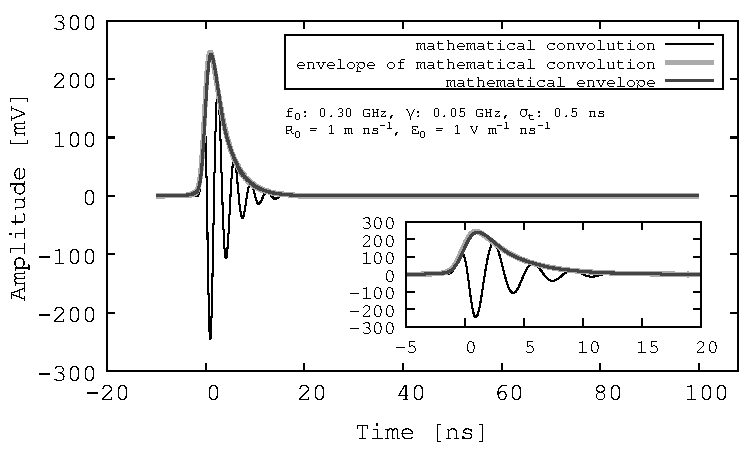
\includegraphics[width=0.5\textwidth]{July3rd_plot1.pdf}
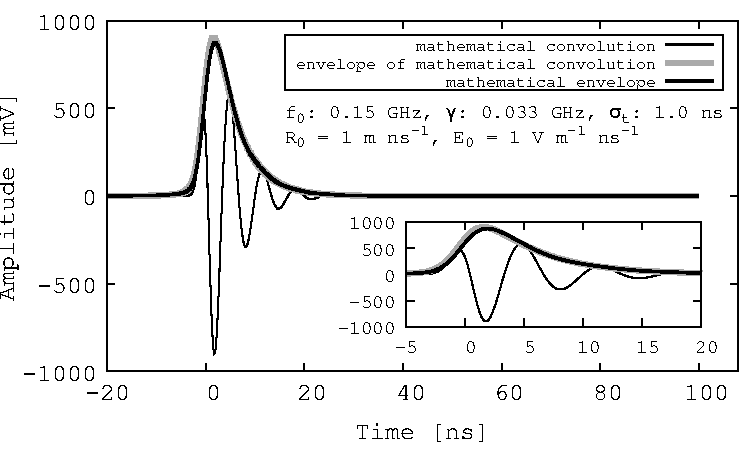
\includegraphics[width=0.5\textwidth]{July3rd_plot2.pdf}
\caption{\label{fig:fig1} (Top) The thin black line represents $s(t) * r(t)$.  The light gray envelope represents the envelope of $s(t) * r(t)$ computed with the Python3 SciPy function scipy.special.hilbert. The dark gray envelope represents Eq. \ref{eq:final}-\ref{eq:final2}. (Bottom) Same as top, for different parameter values.}
\end{figure}
 To demonstrate that \textit{numerical convolution} of $s(t)$ and $r(t)$ produces the same results as the \textit{mathematical convolution} of $s(t)$ and $r(t)$ (Eq. \ref{eq:final3}), the corresponding waveforms are shown in Fig. \ref{fig:fig2}.
\begin{figure}[ht]
\centering
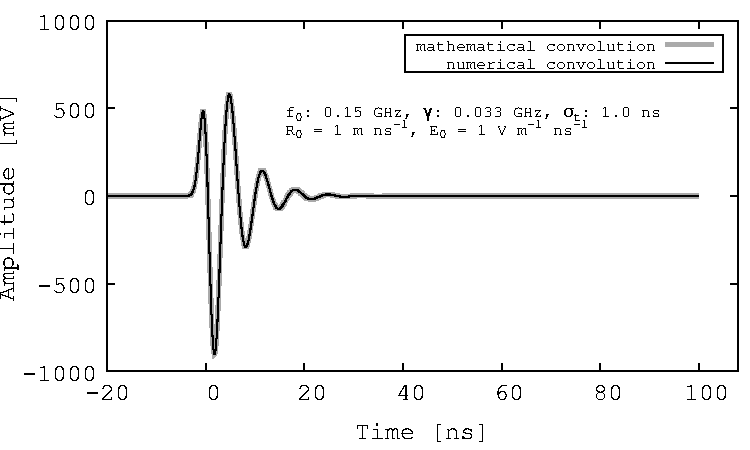
\includegraphics[width=0.5\textwidth]{July7th_plot1.pdf}
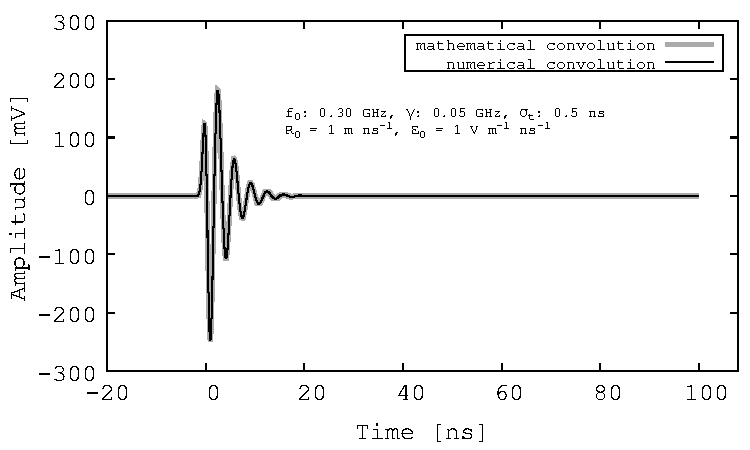
\includegraphics[width=0.5\textwidth]{July7th_plot2.pdf}
\caption{\label{fig:fig2} (Top) The thin black line represents $s(t) * r(t)$, produced using the Python3 SciPy function scipy.signal.convolve. The dark gray line represents Eq. \ref{eq:final3}. (Bottom) Same as top, for different parameter values.}
\end{figure}

\section{Comparison between Analytic Calculations and NuRadioMC}
\label{sec:sim}

\begin{itemize}
\item A data set was generated using NuRadioMC for UHE-$\nu$ interactions in a cylindrical ice volume (see Tab. \ref{tab:1}).  The 100 PeV interactions included charged and neutral electroweak currents, and the LPM effect.  The Askaryan model used to generate the UHE-$\nu$ signals was ARZ2020 \cite{PhysRevD.101.083005}.  ARZ2020 is a semi-analytic parameterization of the Askaryan effect, in which a vector potential $\vec{A}(\vec{r},t)$ is convolved with the profile of the charged particle cascade caused by the UHE-$\nu$ interaction.  ARZ2020 accounts for sub-cascades and the LPM effect, and it has been validated against MC simulations \cite{zhs,10.1103/physrevd.84.103003}.  The Askaryan signal model used in NuRadioMC for this analysis was \textit{not} HH2022 \cite{PhysRevD.105.123019}.  Thus, the correlation between MC output (ARZ2020) and Eqs. \ref{eq:final}-\ref{eq:final2} (HH2022 and this work) is physical.

The detector was \textit{a single string} of 8 RF dipoles.  The ice volume had a depth and radius of 0.65 km and 0.85 km, respectively, and the dielectric properties of the South Pole.  Each RF channel had a filtered, amplified passband of [0.08-1] GHz, and 256 samples at a 1 GHz sampling rate.  The RF trigger responded when any 3 of the 8 voltage traces exceeded $\pm 3 v_{\rm rms}$ of the thermal noise (233K) within a 256 ns window.  The Hilbert envelope of the coherently summed waveform (CSW) was calculated from the traces and correlated against Eqs. \ref{eq:final}-\ref{eq:final2}.  Each correlation was maximized by varying $\sigma_t$.  A rough optimization over a noiseless data set yielded 0.15 GHz and 0.025 GHz for the $f_0$ and $\gamma$ parameters, respectively.  For each signal, a separate thermal noise trace satisfying the RF trigger was generated and correlated against the best-fit analytic envelope.  The results are shown in Fig. \ref{fig:fig3}.

\begin{table}
\centering
\begin{tabular}{| c | c | c |}
\hline
\textbf{Parameter} & \textbf{Value} & \textbf{Note} \\
Ice Model & South Pole & 2015 measurements \\
Signal Model & ARZ2020 & (see \cite{PhysRevD.101.083005}) \\
Trigger & 3 of 8 channels & high-low trigger at $3v_{\rm rms}$ \\
RF channels & 8 & RF bicone (in firn) \\
Noise Temperature & 233K &  \\
Sampling Rate & 1 GHz &  \\
Samples per channel & 256 &  \\
Channel depths & [-4,-6,-8,...-18] m & cable delays included \\
RF cable type & LMR-400 & \\
\hline
\end{tabular}
\caption{\label{tab:1} Important NuRadioMC parameters used in this analysis.}
\end{table}

\begin{figure}
\centering
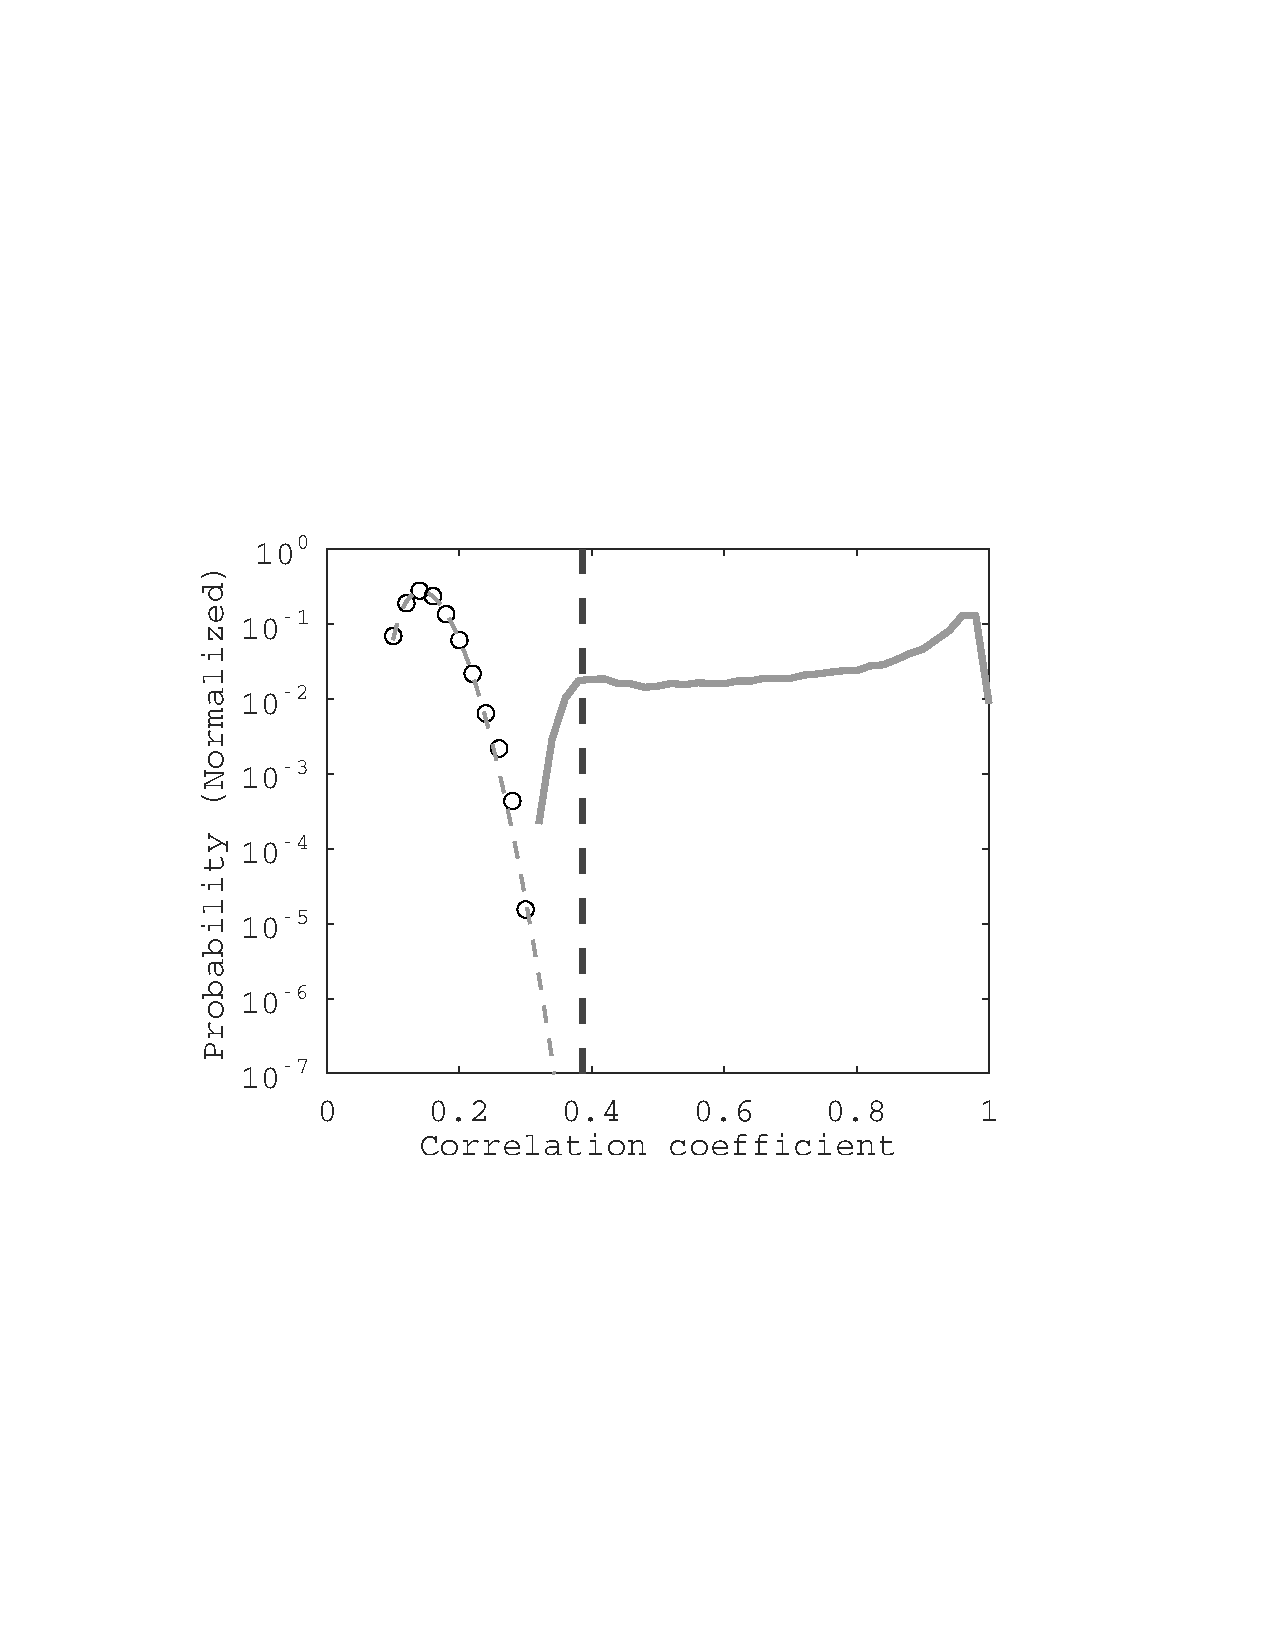
\includegraphics[width=0.5\textwidth,trim=3.25cm 8.25cm 4.5cm 9.0cm,clip=true]{Aug15_plot1.pdf}
\caption{\label{fig:fig3} (Black circles) Noise distribution. (Gray dashed line) Fitting function to noise distribution.  (Solid gray line) UHE-$\nu$ signal distribution.  (Dashed black line) Optimized correlation coefficient threshold value.}
\end{figure}

In Fig. \ref{fig:fig3}, the circles represent the normalized histogram of the correlation coefficent between the optimized analytic envelope and thermal noise.  A fitting function of the form $x^2 \exp(-0.5 x^2)$ was fit to the noise distribution, and is represented by the gray dashed line.  The solid gray line represents the signal distribution, which peaks at a correlation value of 0.94.  Lower signal correlation values correspond to lower SNR values (Fig. \ref{fig:fig4}).  The vertical black dashed line represents a threshold of 0.4.  For the simulated UHE-$\nu$, 99.99\% of correlations between CSWs and analytic envelopes are greater than or equal to this threshold.  Assuming a thermal trigger rate of 1 Hz, integrating the PDF of the noise distribution above the correlation threshold is equivalent to 0.2 noise events every 5 years.  An example CSW fit by the analytic envelope is shown in Fig. \ref{fig:example_waveforms}.

\begin{figure}
\centering
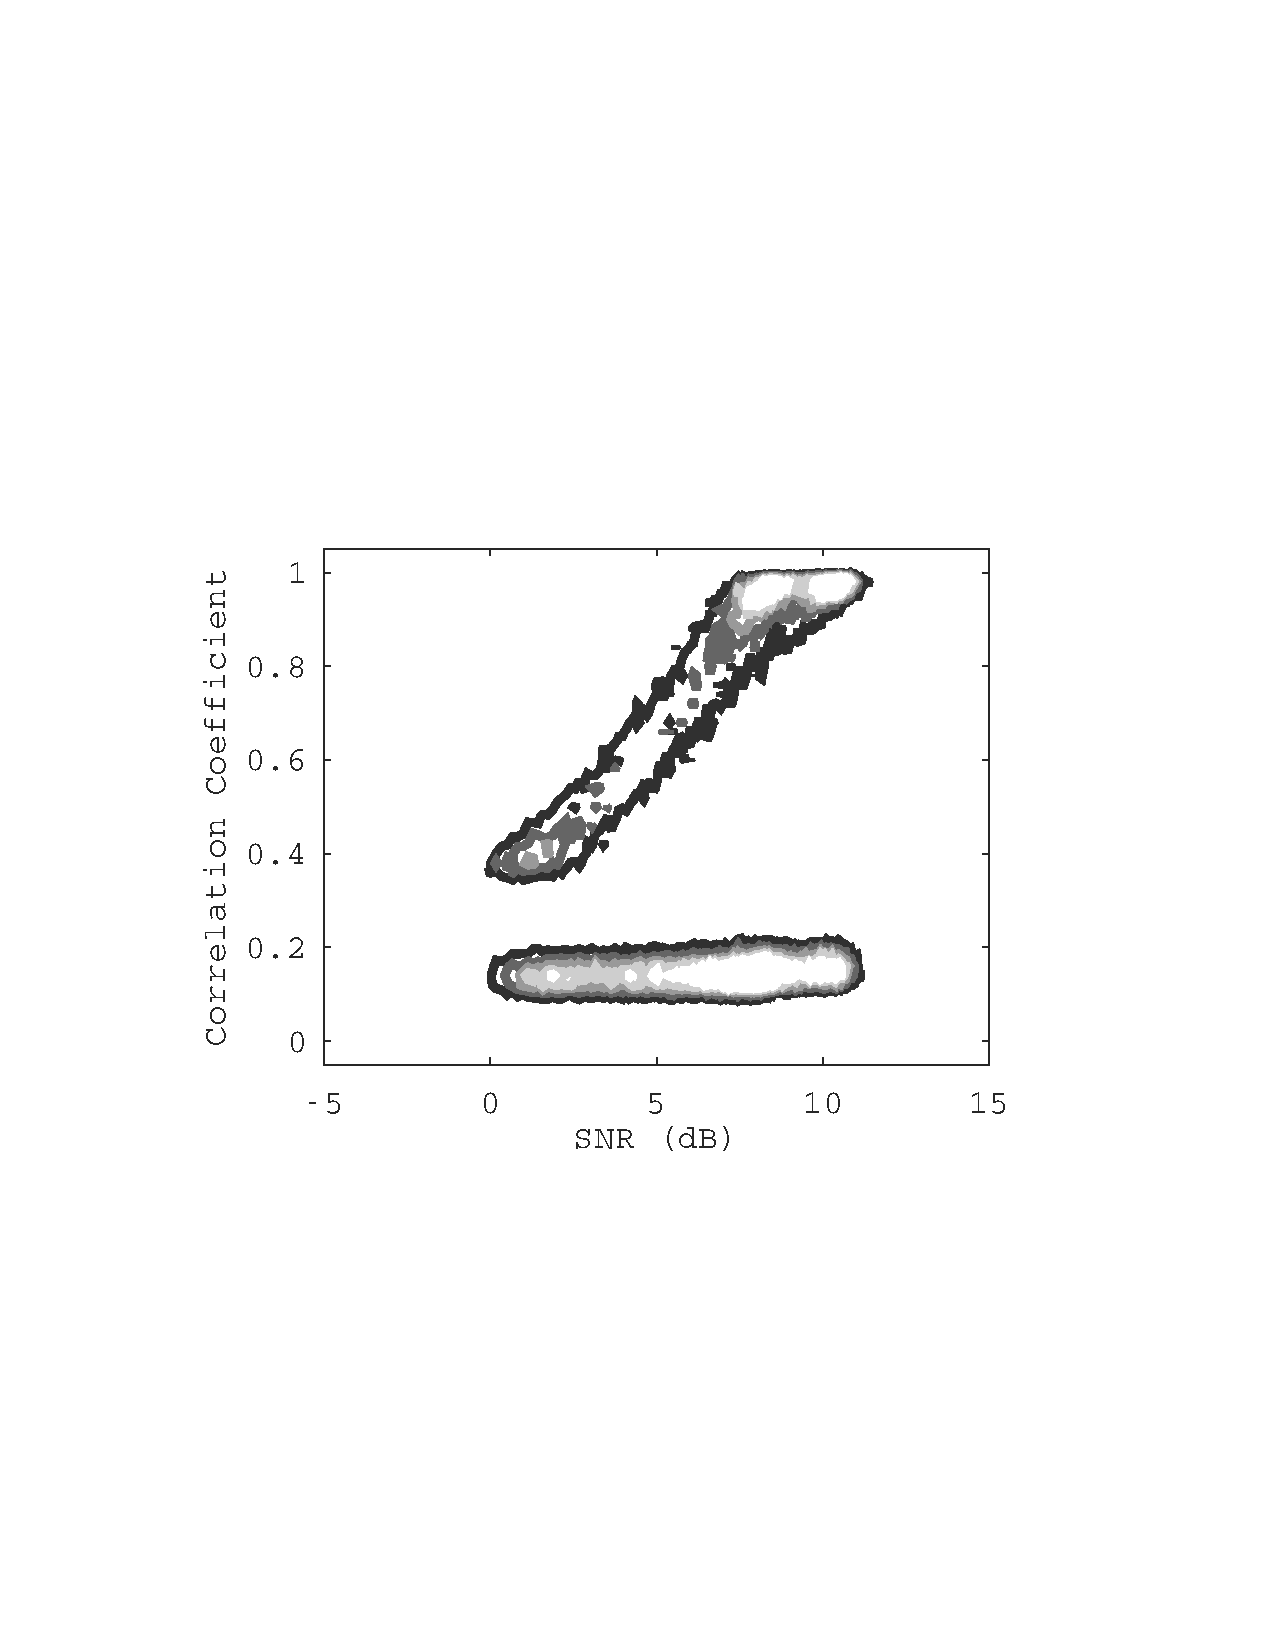
\includegraphics[width=0.5\textwidth,trim=3.25cm 8.25cm 4.5cm 9.0cm,clip=true]{Aug15_plot2.pdf}
\caption{\label{fig:fig4} The correlation versus SNR (dB) for UHE-$\nu$ signals (upper distribution) and RF thermal noise (lower distribution).  Color scale: normalized histogram value, with five equally spaced contours between 0.0 and 0.002.}
\end{figure}

\begin{figure}
\centering
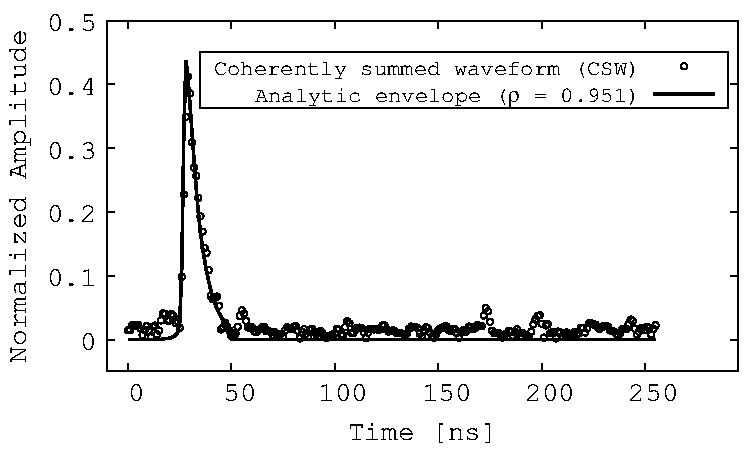
\includegraphics[width=0.5\textwidth]{Sept25_plot1.pdf}
\caption{\label{fig:example_waveforms} A single-pulse CSW signal (black dots) from a 100 PeV UHE-$\nu$, matched to an analytic envelope (thick black line) with a correlation coefficient $\rho = 0.951$.}
\end{figure}

The correlation between the optimized analytical envelope and UHE-$\nu$ signals depends on the signal to noise ratio (SNR).  Let $v_{\rm pp}$ and $v_{\rm rms}$ represent the peak-to-peak and rms values a voltage traces, respectively.  The SNR, in decibels, is defined as

\begin{equation}
\snr_{\rm dB} = 20\log_{10}\left(\frac{1}{2}\frac{v_{\rm pp}}{v_{\rm rms}}\right)
\end{equation}

In Fig. \ref{fig:fig4}, the correlation coefficient is plotted versus the SNR in dB for the data shown in Fig. \ref{fig:fig3}.  The upper and lower distributions correspond to CSWs from UHE-$\nu$ events and thermal noise, respectively.  All RF thermal noise events satisfy the station trigger ($\pm 3v_{\rm rms}$ HL threshold).  The correlation coefficient for UHE-$\nu$ events is proportional to SNR$_{\rm dB}$, while the correlation coefficient for thermal noise is independent of SNR$_{\rm dB}$.  Note that the SNR of a CSW does not equal the SNR of the individual voltage traces.  Rather, the individual voltage traces will have SNR values approximately 5-10 dB \textit{lower} than the CSW SNR.  If $N$ voltage traces contain signal, computing the CSW raises the linear SNR by a factor of $\sqrt{N}$, and adds to the SNR in dB a factor of $20\log_{10}(N)$.  For an event with 3 of 8 channels containing signal, $20\log_{10}(3)\approx 5$ dB, while $20\log_{10}(8)\approx 9$ dB.  The exact increase depends on how many RF channels contain signal.

\begin{figure}
\centering
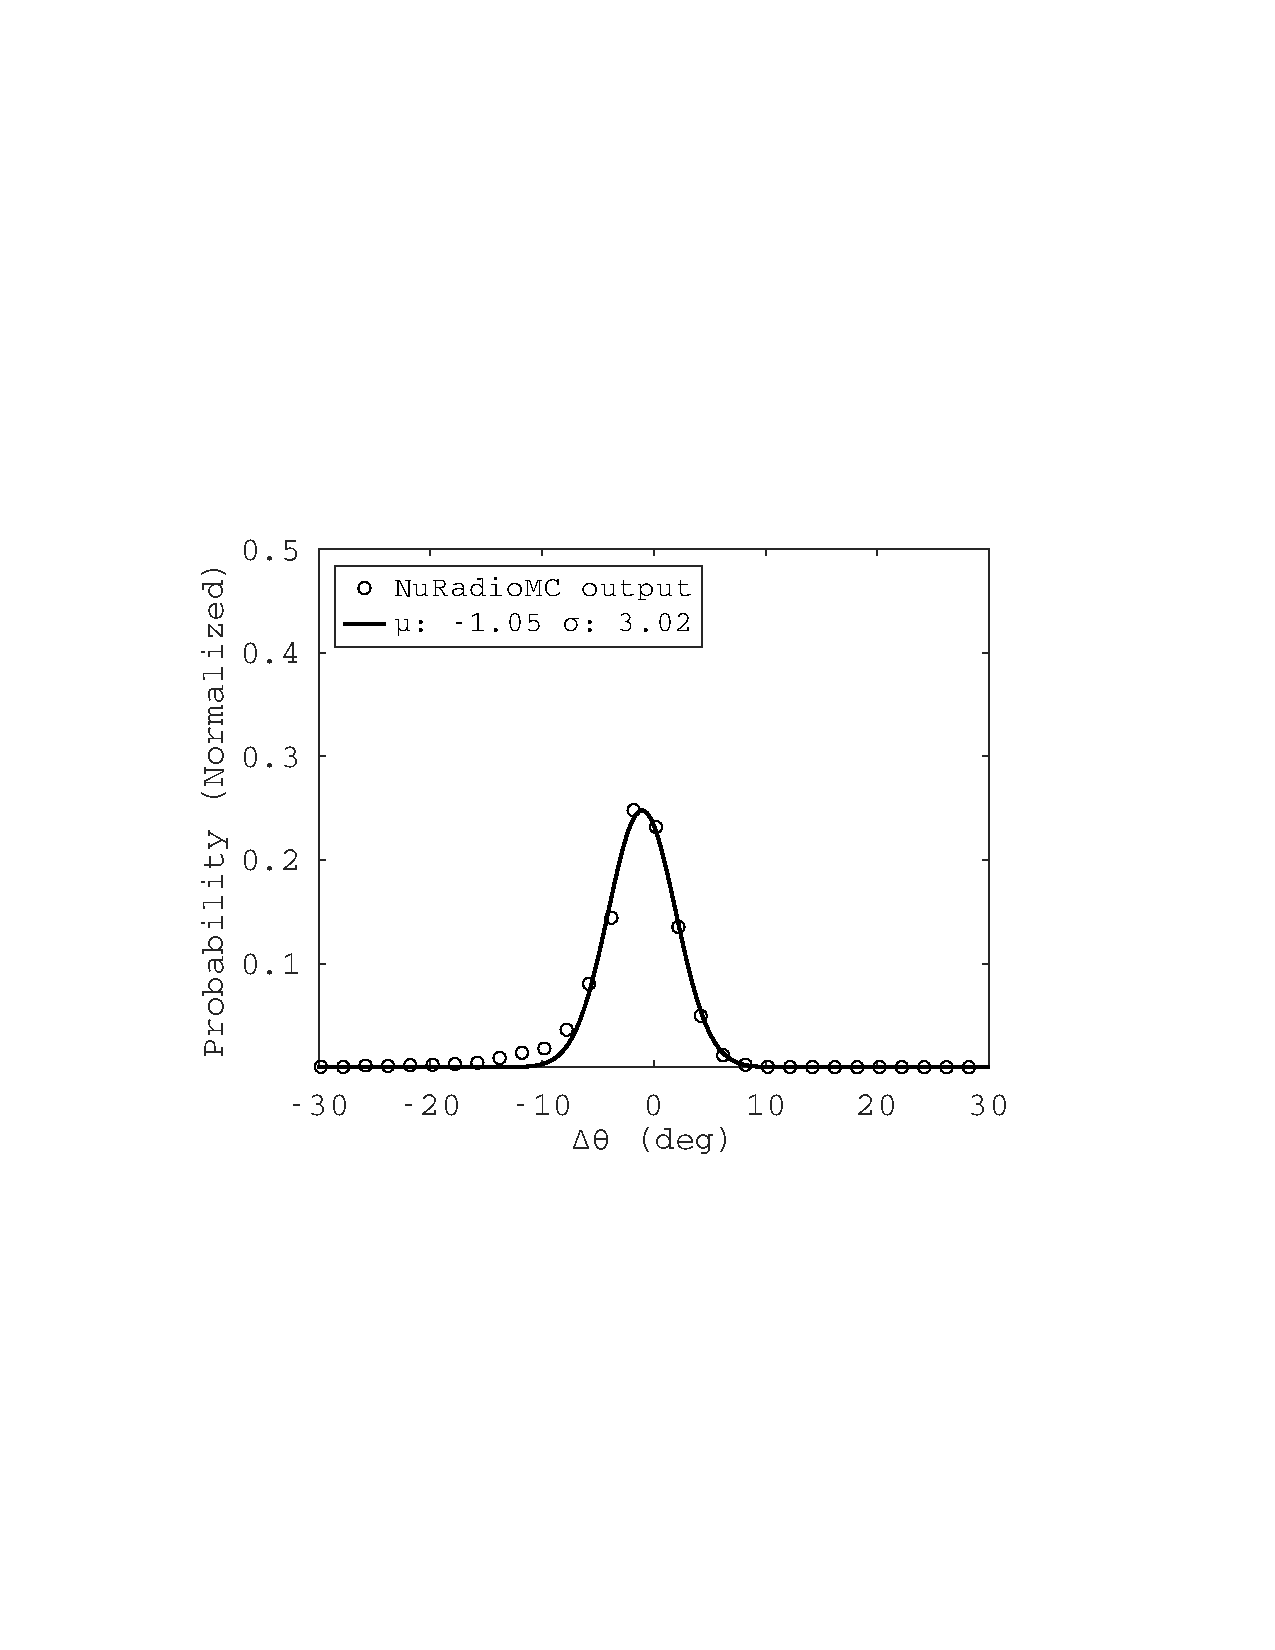
\includegraphics[width=0.5\textwidth,trim=3.25cm 8.25cm 4.5cm 9.0cm,clip=true]{Aug18_plot1.pdf}
\caption{\label{fig:fig5} (Black circles) Viewing angle from NuRadioMC. (Solid black line) Gaussian fit, with $\mu = -1.05$ deg, and $\sigma = 3.02$ deg.  (Black dashed line) Cherenkov angle, $\theta_{\rm C}$.}
\end{figure}

\item Equations \ref{eq:uncert}-\ref{eq:a_err} may be used to reconstruct the natural logarithm of the UHE-$\nu$ cascade energy, $\ln\Lambda$.  For Eq. \ref{eq:uncert}, $\sigma_t$ is measured from the optimized analytic envelope, $c$ and $\theta_{\rm C}$ are known constants, and an assumption must be made for $\Delta\theta$.  We will make the assumption that $\Delta\theta \approx \Delta\theta_{\rm rms}$.  The assumption is justified since the $\Delta\theta$ distribution is Gaussian.  The MC truth for $\Delta\theta$ in this analysis is shown in Fig. \ref{fig:fig5}, with a Gaussian fit ($\mu=-1.05$ deg, $\sigma=3.02$ deg).  The rms and the $\sigma$ parameter are equal for Gaussian distributions with zero mean, so we let $\Delta\theta \to \Delta \theta_{\rm rms}$.  The fractional error $\sigma_{\Delta\theta}/\Delta\theta$ is then set to 1.0, reflecting uncertainty in this parameter.  Solving Eq. \ref{eq:uncert} for $a$ gives

\begin{equation}
a = \frac{c\sigma_t}{\Delta\theta_{\rm rms} \sin\theta_{\rm C}}
\end{equation}

The result for the fractional error in $a$ is found by propagating error from $\sigma_t$ and $\Delta\theta$, defined as $\epsilon$ and $\sigma_{\Delta\theta}$, respectively.  The result is

\begin{equation}
\frac{\sigma_a}{a} = \left(\left(\frac{\epsilon}{\sigma_t}\right)^2 +  \left(\frac{\sigma_{\Delta\theta}}{\Delta\theta}\right)^2\right)^{1/2}
\end{equation}

The first term is small compared to the second, as it is limited by the scan resolution for $\sigma_t$ and the number of samples per analytic envelope.  The scan resolution is set to 0.2 ns in the optimization, and there are typically $>10$ samples per envelope, or about 10 ns.  Thus, $\left(\epsilon/\sigma_t\right)^2$ is two orders of magnitude smaller than $\left(\sigma_{\Delta\theta}/\Delta\theta\right)^2$, so

\begin{equation}
\frac{\sigma_a}{a} = \left|\frac{\sigma_{\Delta\theta}}{\Delta\theta}\right| = \left|\frac{\Delta\theta_{\rm rms}}{\Delta\theta_{\rm rms}}\right|\approx 1
\end{equation}

Setting the ratio to 1 reflects the idea that the rms is equal to $\sigma$ for a normal distribution.  Inserting this assumption into Eq. \ref{eq:a_err} gives

\begin{equation}
\frac{\sigma_{\ln\Lambda}}{\ln\Lambda} \approx 2 \label{eq:a_err_2}
\end{equation}

Using Eqs. \ref{eq:em} and \ref{eq:had}, the logarithm of the energy is

\begin{equation}
\ln\Lambda = \left( \frac{c\sigma_t}{c_{\rm em/had} \Delta\theta_{\rm rms}\sin\theta_{\rm C}} \right)^2 \label{eq:lnLambda}
\end{equation}

Using Eqs. 10 and 12 from HH2022 (\cite{PhysRevD.105.123019}), $c_{\rm em}$ and $c_{\rm had}$ were found to be 0.80 and 0.93 meters, respectively (FWHM, $R=0.5$).  Using Eq. \ref{eq:lnLambda}, the $\sigma_t$ results from the optimized envelope fits to UHE-$\nu$ signal CSWs may be used to deduce the logarithm of the UHE-$\nu$ cascade, $\log_{10} E_{\rm C}$.  First, converting to the base-10 logarithm introduces a factor of $\ln(10)$ in the denominator of Eq. \ref{eq:lnLambda}.  Second, $\ln\Lambda = \ln(E_{\rm C}/E_{\rm crit})$, where $E_{\rm C}$ is the cascade energy, and $E_{\rm crit}\approx 10^8$ eV is known as the critical energy \cite{PhysRevD.105.123019}.  Since $\ln\Lambda = \ln E_{\rm C} - \ln E_{\rm crit}$, separating this ratio adds a constant to the right hand side of Eq. \ref{eq:lnLambda}.  Third, let $c_{\rm ave}$ be the average of $c_{\rm em}$ and $c_{\rm had}$, reflecting the unknown hadronic or electromagnetic nature of the cascade.  The modified form of Eq. \ref{eq:lnLambda} is

\begin{equation}
\log_{10} E_{\rm C} = \frac{\left( c\sigma_t \right)^2}{\ln 10(c_{\rm ave} \Delta\theta_{\rm rms}\sin\theta_{\rm C})^2} + \log_{10} E_{\rm crit} \label{eq:lnLambda_2}
\end{equation}

Table \ref{tab:2} contains the preliminary results for the reconstruction of $\log_{10}E_{\rm C}$.  The results are consistent with the MC truth.  Note that when applying the change of base formula, factors of $\ln(10)$ cancel in the error ratio of Eq. \ref{eq:a_err_2}, so the error in $\log_{10} E_{\rm C}$ remains $2.0$.  The $\sigma_t$ result is the average value of optimized analytic envelopes fit to signal CSWs generated by 15133 UHE-$\nu$ events that triggered the detector with $E_{\rm C} = 100$ PeV.  Note that the error in the \textit{average} $\sigma_t$ over all events fluctuates due to varying $\Delta\theta$, while the error in \textit{individual} $\sigma_t$ per CSW fit is negligible if the samples per CSW is much greater than 1.  By far, the largest sources of systematic error are \textit{reflected signals} in the CSWs.

Reflected signals are caused when more than one ray-tracing solution is available between the Askaryan radiation source and the detector.  Signals that propagate directly to the detector are known as \textit{direct signals}, while signals that first reflect at the snow-air interface, or in the glacial firn, are known as \textit{reflected signals}.  Complex RF signal propagation in polar ice has been studied, and even proposed as a UHE-$\nu$ energy reconstruction technique \cite{Barwick:2018497,anker2019neutrino-734}.  When \textit{direct} and \textit{reflected} signals both arrive at the detector, recorded voltage traces contain both direct and reflected signals.  The analytic envelope, however, assumes a single pulse.  Thus, direct and reflected pulses that overlap, or are closely spaced, yield larger $\sigma_t$ values than the average quoted in Tab. \ref{tab:2}.  This effect systematically overestimates the $\log_{10} E_{\rm C}$.  An example of a CSW event with direct and reflected components fit by an analytic envelope is shown in Fig. \ref{fig:example_waveforms_2}.

\begin{table}
\centering
\begin{tabular}{| c | c |}
\hline
\textbf{Parameter} & \textbf{Average Value} \\ \hline
MC Truth, $E_{\rm C}$ [eV] & $10^{17}$ \\
MC Truth, $\log_{10}E_{\rm C}$ & $17$ \\
$c$ & $0.3/1.78$ m ns$^{-1}$ \\
$\overline{\sigma_t}$ & $1.229 \pm 0.004$ ns \\
$c_{\rm ave}$ & 0.86 m \\
$\Delta\theta_{\rm rms}$ & $3.78\pm0.04$ degrees \\
$E_{\rm crit}$ & 100 MeV \\
$\sin\theta_{\rm C}$ & 0.8271 \\ \hline
\textbf{Reconstructed} $\mathbf{\log_{10}E_{\rm C}}$ & $16.5\pm 2.0$ \\
\hline
\end{tabular}
\caption{\label{tab:2} Energy reconstruction parameters used to calculate the logarithm of the UHE-$\nu$ cascade energy, $\log_{10}E_{\rm C}$.}
\end{table}

\begin{figure}
\centering
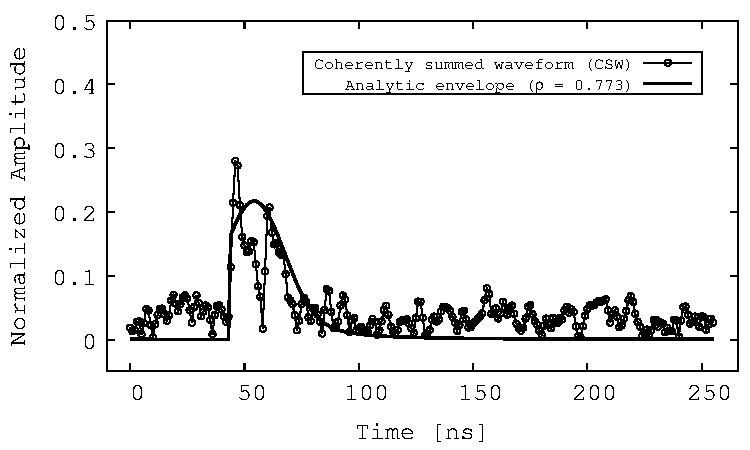
\includegraphics[width=0.5\textwidth]{Sept25_plot2.pdf}
\caption{\label{fig:example_waveforms_2} A direct and reflected CSW signal (black dots and thin black line) from a 100 PeV UHE-$\nu$, matched to an analytic envelope (thick black line) with a correlation coefficient $\rho = 0.773$.}
\end{figure}

\end{itemize}

\section{Conclusion}
\label{sec:conc}

The conclusion.

\appendix

\section{Details}
\label{app:a}

The details.

\bibliography{apssamp}

\end{document}

